\documentclass{article}

% Set page margin
% http://kb.mit.edu/confluence/pages/viewpage.action?pageId=3907057
\usepackage[margin=2.5cm]{geometry}

% Math operations
\usepackage{amsmath}

% FloatBarrier
\usepackage{placeins}

% Insert images from file path
\usepackage{graphicx}
\usepackage{wrapfig}

\usepackage{caption}

% Mono spaced font
\usepackage{bera}

% Referencing figures, listings etc. 
\usepackage{hyperref}
\usepackage{capt-of}

% some color definitions
\usepackage{xcolor}
\definecolor{cblue}{RGB}{16,78,139}
\definecolor{cred}{RGB}{139,37,0}
\definecolor{cgreen}{RGB}{0,139,0} 
\definecolor{corange}{RGB}{255,160,77}
\definecolor{clightblue}{RGB}{62,137,190}

% normal box
\newcommand{\sqboxs}{1.2ex}% the square size
\newcommand{\sqboxf}{0.6pt}% the border in \sqboxEmpty
\newcommand{\sqbox}[1]{\textcolor{#1}{\rule{\sqboxs}{\sqboxs}}}

% Code highlighting
\usepackage{color}
\usepackage{listings}
\usepackage{setspace}

% Define colors for Python listings
\definecolor{Code}{rgb}{0,0,0}
\definecolor{Decorators}{rgb}{0.5,0.5,0.5}
\definecolor{Numbers}{rgb}{0.5,0,0}
\definecolor{MatchingBrackets}{rgb}{0.25,0.5,0.5}
\definecolor{Keywords}{rgb}{0,0,1}
\definecolor{self}{rgb}{0,0,0}
\definecolor{Strings}{rgb}{0,0.63,0}
\definecolor{Comments}{rgb}{0,0.63,1}
\definecolor{Backquotes}{rgb}{0,0,0}
\definecolor{Classname}{rgb}{0,0,0}
\definecolor{FunctionName}{rgb}{0,0,0}
\definecolor{Operators}{rgb}{0,0,0}
\definecolor{Background}{rgb}{0.98,0.98,0.98}

\lstdefinelanguage{Python}{
	numbers=left,
	numberstyle=\footnotesize,
	numbersep=1em,
	xleftmargin=1em,
	framextopmargin=2em,
	framexbottommargin=2em,
	showspaces=false,
	showtabs=false,
	showstringspaces=false,
	frame=l,
	tabsize=4,
	% Basic
	basicstyle=\ttfamily\small\setstretch{1},
	backgroundcolor=\color{Background},
	% Comments
	commentstyle=\color{Comments}\slshape,
	% Strings
	stringstyle=\color{Strings},
	morecomment=[s][\color{Strings}]{"""}{"""},
	morecomment=[s][\color{Strings}]{'''}{'''},
	% keywords
	morekeywords={import,from,class,def,for,while,if,is,in,elif,else,not,and,or,print,break,continue,return,True,False,None,access,as,,del,except,exec,finally,global,import,lambda,pass,print,raise,try,assert},
	keywordstyle={\color{Keywords}\bfseries},
	% additional keywords
	morekeywords={[2]@invariant,pylab,numpy,np,scipy},
	keywordstyle={[2]\color{Decorators}\slshape},
	emph={self},
	emphstyle={\color{self}\slshape},
	%
}
\linespread{1.3}


% Define new float types so that I can reference them with captionof from the capt-of package. 
% https://tex.stackexchange.com/questions/6157/floating-an-algorithm
% Could be helpful as well: https://tex.stackexchange.com/questions/115499/image-caption-within-newfloat
\usepackage{float}
\newfloat{MyListing}{t}{lop}
\newfloat{Enumerate}{t}{lop2}


\begin{titlepage}
	\title{Assignment 1 - Ridge Regression and Model Selection\\
		{\large Course: \textit{Advanced Machine Learning}}}
	\date{\today}	
\end{titlepage}




\begin{document}

\maketitle

\section{Teammembers and Contributions}
\label{sec:TeammembersAndContributions}

\begin{itemize}
	\item \makebox[0.4\linewidth]{\textbf{Bernd Menia}, \hfill\textit{01316129}:} Report, Part Programming
	\item \makebox[0.4\linewidth]{\textbf{Maximilian Samsinger}, \hfill\textit{01115383}:} Main Programming
\end{itemize}

\noindent The difference in our contributions is because Bernd just only started working with Machine Learning, while Maximilian has already prior knowledge in the subject. Thus we worked together, but the main programming work for this assignment was done by Maximilian. Apart from that due to the size of the code we will only list the important parts and explain them in detail with the results. 

\section{Prerequisites and Creation of Subsets} 
\label{sec:PrerequisitesAndCreationOfSubsets}
\begin{wrapfigure}{R}{0.5\textwidth} %this figure will be at the right
	\centering
	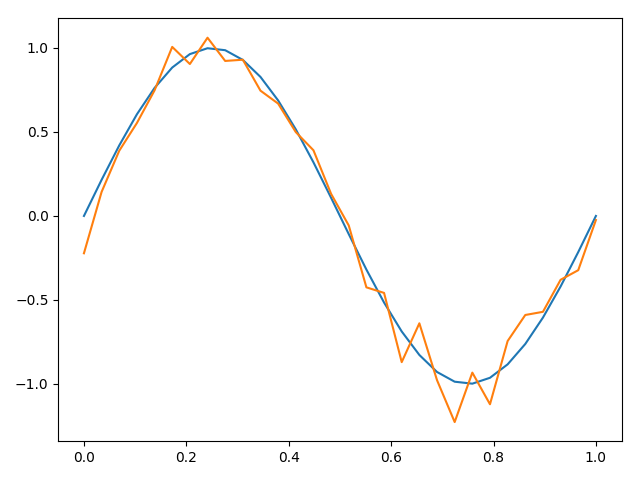
\includegraphics[width=0.5\textwidth]{plots/sine5.png}
	\caption{Initial sine function}
	\sqbox{clightblue} Only $\sin(2*\pi*x)$\\
	\sqbox{corange} Including randomized errors
	\label{plot:sine5}
\end{wrapfigure}

Our data points are denoted by $N$ which we set to 30. There was no mathematical reason for this, but by testing our code with multiple values for $N$ we found 30 to be a fitting number for this assignment. The nonlinear function that we used as the starting point for this assignment, $f(x) = \sin(2*\pi*x)$, can be seen in \autoref{plot:sine5}. We chose a sine function because it is simplistic and let's us demonstrate the linear regression easily. The blue curve corresponds to the initial sine function whereas the orange curve depicts the calculated values including the randomized errors. \\

\FloatBarrier

%TODO What happens with the k-fold cross-validation when not all buckets have the same amount of elements? 

\noindent The next step is to divide our data points into training- and test sets. We chose to use $\frac{N}{K}$, where $K = 5$ of all data points rounded down. There is no rule how the points have to be distributed. This also means that we can theoretically distribute the points like we want. Let's assume we have a vector $x$ that holds all x-values for the training- and test points. We could take the first $2$ elements of the vector for the trainings set and the rest for the test set. However this would most likely be very bad because if the elements are ordered we have a biased test set. Taking the first 2 elements of $[1,2,3,4,5,6,7,8,9,10,11,12]$ would give $[1,2]$ which is heavily biased towards lower x-values, or rather the left side of the function. In that case it can happen that the error function produces a biased (i.e. high) result as well. \\
\\
A simple solution would be to order the vector and then re-do the explained procedure. However even by doing this there is the possibility that the points are not evenly distributed nevertheless and therefore stay biased. Randomizing $x$ could still produce the result $[1,2,5,3,12,7,8,4,10,9,2,6,11]$ in which case the trainings points would again be $[1,2]$, which is not desirable. \\
\\
There is another solution that fixes this problem without much trouble. First we have to order our vector $x$ and then divide it into $\frac{N}{K}$ subsets. For example if $N = 12$ and $K = 3$ then we would split $x$ into $\frac{12}{3} = 4$ as equally big parts as possible. For $x$ this would result in $[[1,2,3],[4,5,6],[7,8,9],[10,11,12]]$. The second step is to randomize each of these subsets. This could for example result in $[[3,1,2],[5,4,6],[7,8,9],[11,10,12]]$. Finally we can take some elements out of different subsets as our test points and the rest as our trainings points. Doing this we can guarantee that there is no bias towards any part of the curve because the subsets are evenly distributed over the x-values.


\section{K-Fold Cross-Validation}
\label{sec:K-FoldCrossValidation}
%Doing this is also convenient because we can use the subsets for our K-Fold Cross-Validation. Since we have $\frac{N}{K} = I$ subsets, we iterate I times over all elements in the following way: We start at $i = 0$ up to $i = I-1$ and take the $i-th$ subset as our test points. All other subsets correspond to the training points for each iteration respectively. In other words: Each iteration is one fold. So taking our example from before, $[[3,1,2],[5,4,6],[7,8,9],[11,10,12]]$, we can produce 4 different folds. If $i = 0$ then we would take the first subset, $[3,1,2]$, as our test points and all other subsets, $[5,4,6],[7,8,9],[11,10,12]$, as our training points. If $i = 1$ then our test points would correspond to the second subset, [5,4,6], whereas the training points would be $[3,1,2],[7,8,9],[11,10,12]$ and so on. Finally we simply take the average of all folds as our result. How this is done will be explained in the next section. 

Doing this is also convenient because we can use the subsets for our K-Fold Cross-Validation. The only adaptation that we have to do is to iterate K times over our subsets and put the $k-th$ element of each subset in a new subset. Let's take a look at our example from before, $[[3,1,2],[5,4,6],[7,8,9],[11,10,12]]$. In the first iteration, $k=0$, we take the first element of each subset and obtain $[3,5,7,11]$, in the second iteration we take each second element and so on. Overall we now have a new set of $K$ subsets: $[[3,5,7,11],[1,4,8,10],[2,6,9,12]$. What we can see here is that each subset has a mix of different parts of values and no biases, which is good. \\
\\
Now we can take those subsets and iterate over them again to calculate our folds. For this we iterate $\frac{N}{K} = I$ times over all elements in the following way: We start at $i = 0$ up to $i = I-1$ and take the $i-th$ subset as our test points. All other subsets correspond to the training points for each iteration respectively. In other words: Each iteration is one fold. So taking our example from before, $[[3,5,7,11],[1,4,8,10],[2,6,9,12]]$, we can produce 3 different folds. If $i = 0$ then we would take the first subset, $[3,5,7,11]$, as our test points and all other subsets, $[1,4,8,10],[2,6,9,12]$, as our training points. If $i = 1$ then our test points would correspond to the second subset, $[1,4,8,10]$, whereas the training points would be $[3,5,7,11],[2,6,9,12]$ and so on. Finally we simply take the average of all folds as our result. How this is done will be explained in the next section. 


\section{Calculation of the Results}
\label{sec:CalculateTheResults}
With that in mind it is now time to calculate the actual results. To dampen the effect of high amplitudes, due to possible outliers, we included a regularization factor, $\lambda$, in our calculations. The range of our $\log(\lambda)$ values is divided into 300 elements, ranging from -37 up to -1 in equal steps. For each $\lambda$ we calculate the training- and test errors, as well as the coefficients of our resulting functions with the K-Fold Cross Validation as seen in \autoref{sec:K-FoldCrossValidation}. All resulting values then get sorted. \\
\\
From there on we chose 3 specific curves to showcase the effect of \textbf{underfitting}, \textbf{overfitting} and \textbf{optimal fitting}. For the underfitting curve we chose the $\lambda$ value were the error for the training set was the highest. On the contrary the overfitting curve is represented by the $\lambda$ value that has the lowest training error, but a comparatively high test error. Finally the optimal fitting curve is simply the curve with the lowest combined training- and test error, i.e. the best approximation to our initial function. All three curves can be seen in \autoref{plot:full4cropped}, together with the actual underlying function, the randomized data points and the initial sine function from which we approximated our results.  

\begin{figure}[h]
	\centering
	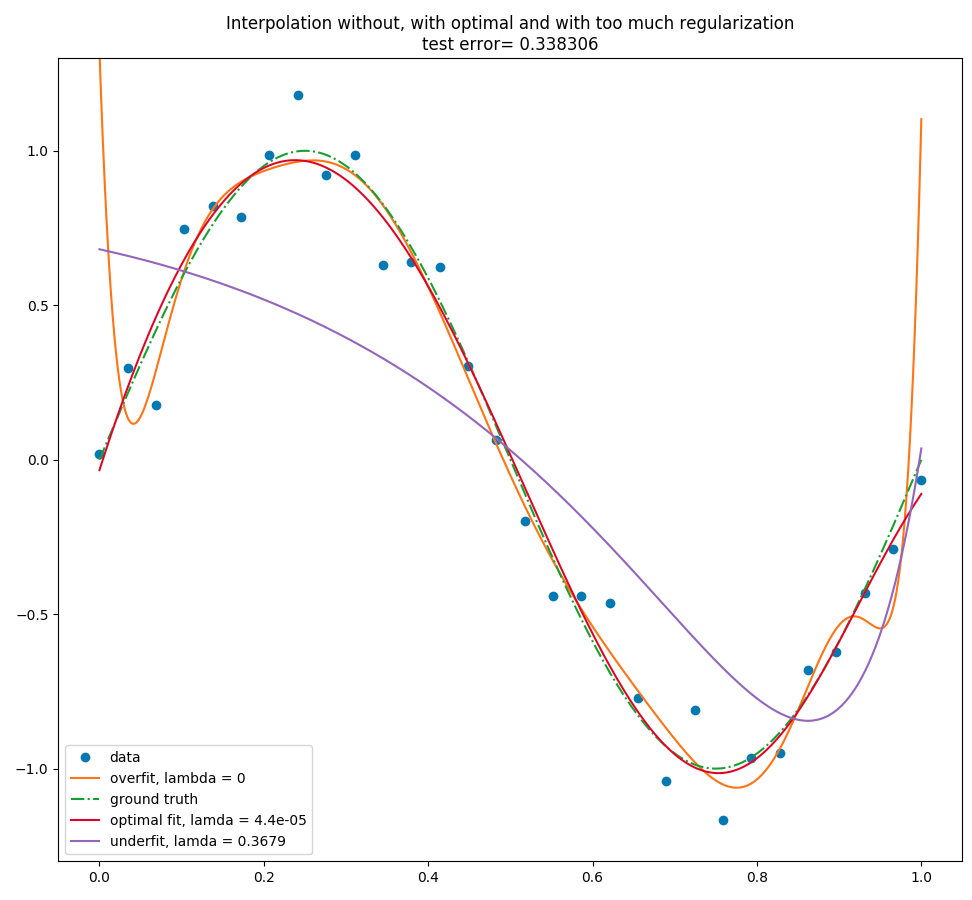
\includegraphics[width=0.9\linewidth]{plots/full4cropped.png}
	\caption{Various results with different $\lambda$ values. }
	\label{plot:full4cropped}
\end{figure}


\newpage
\section{Error Ratio}

\begin{wrapfigure}{R}{0.45\textwidth} %this figure will be at the right
	\centering
	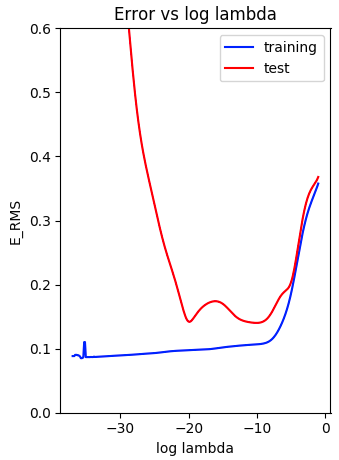
\includegraphics[width=0.45\textwidth]{plots/error4cropped.png}
	\caption{Ratio between the test- and training errors}
	\label{plot:error4cropped}
\end{wrapfigure}

The ratio between the test- and training errors can be seen in \autoref{plot:error4cropped}. Note that we have taken the natural logarithm of the $\lambda$'s so that we can properly display all values in a small plot. As we can see the more we go to the left of our graph, i.e. the $\lambda$ values get smaller, the overfitting increases drastically. The error for the training set stays almost the same from about $-8$ to $-37$, however from $-20$ downwards the test errors skyrocket. This represents overfitting of our initial function and can also be seen as the orange curve in \autoref{plot:full4cropped}. The bump between $-20$ and $-10$ is interesting, but after having run the program multiple times with results that produced no bumps we think it's just a coincidence. \autoref{plot:error4cropped} also shows us underfitting on the right side of the plot. From about $-8$ up to $0$ we can again see that the test errors skyrocket. However in contrast to overfitting, due to the nature of underfitting curves, the training errors also increase. This happens because we try to fit a lower order function to a higher order one of which it simply cannot follow the ups and downs. \\
\\
Finally it has to be noted that we use randomized functions to test our program. So the $\lambda$ values of the curves and the curves themselves may change each run. For example another run of the program yields the results as seen in \autoref{plot:full5}.

\begin{figure}[h]
	\centering
	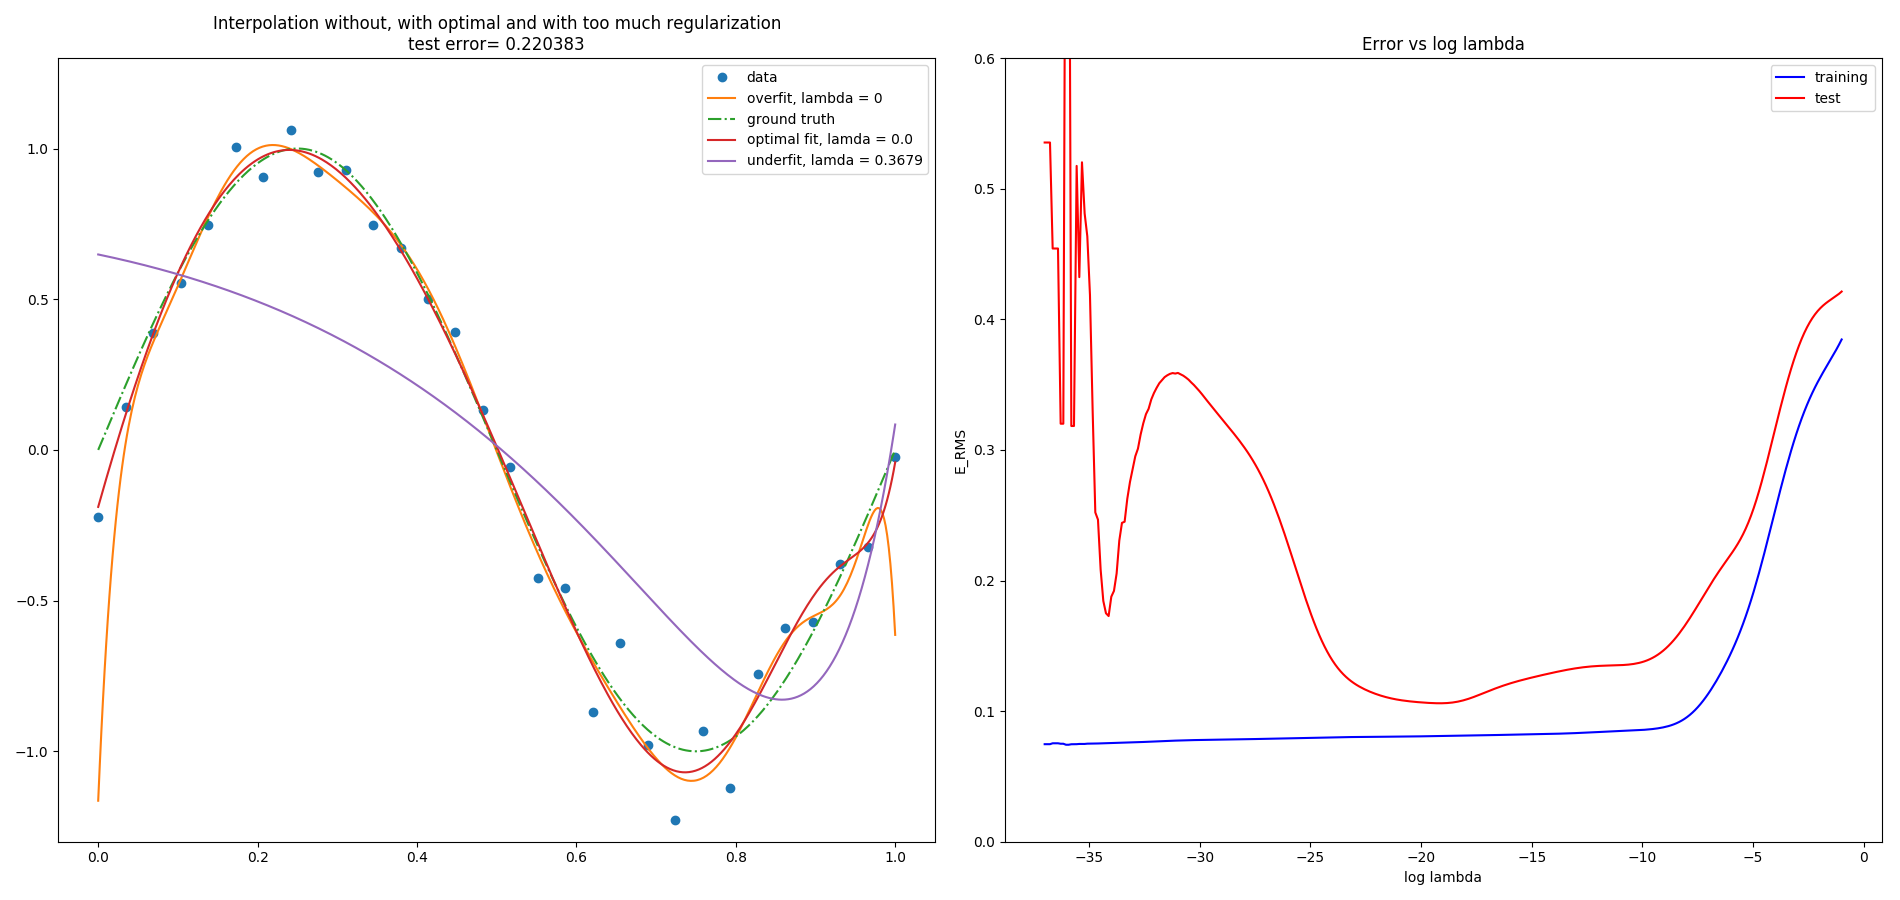
\includegraphics[width=\linewidth,height=6.1cm]{plots/full5.png}
	\caption{Another randomized run through with various results.}
	\label{plot:full5}
\end{figure}
	
\end{document}